\documentclass[10pt]{article}
\usepackage[T1]{fontenc}
\usepackage[utf8]{inputenc}
\usepackage[spanish,es-tabla]{babel}
\usepackage[margin=1.8cm]{geometry}
\usepackage{graphicx}
\usepackage{booktabs}
\usepackage{tabularx}
\usepackage{array}
\usepackage{float}
\usepackage{caption}
\usepackage{enumitem}
\usepackage[protrusion=true,expansion=false]{microtype}
\usepackage{xcolor}
\usepackage{amsmath}

\setlength{\parindent}{0pt}
\setlength{\parskip}{4pt}
\captionsetup{font=small,labelfont=bf,skip=4pt}

\newcommand{\sincaptura}{\textit{Sin captura.}}
\newcommand{\cod}[1]{\texttt{#1}}

\begin{document}

\begin{center}
  {\Large\bfseries AP-U1 · AforoSeguro: control de aforo distribuido}\\[3pt]
  {\large Informe de ejecución y análisis}\\[8pt]
  Bryan Humberto Lombeida Escaleras\\
  Aplicaciones Distribuidas (ISR-701) · 23 de noviembre de 2026
\end{center}

\section{Alcance del prototipo y evidencia disponible}

AforoSeguro se organiza como un coordinador central (identificador 0) y tres
puertas: P1 Norte, P2 Sur y P3 Este (identificadores 1, 2 y 3). La comunicación
se plantea con Java RMI: la interfaz \cod{ICoordinadorRemoto} expone
\cod{procesar(Solicitud)} y las clases \cod{Solicitud} y \cod{Respuesta} son
serializables. RMI se encarga de la conexión TCP, de la delimitación de los
mensajes y de transportar los objetos por copia; el programa no tiene que
construir el \emph{framing}. La configuración está en \cod{config.properties}
(aforo máximo 10, token de acceso, host \cod{127.0.0.1} y puertos 5000 y 5001).

El diseño del coordinador contempla un contador global \cod{dentro}, la
validación del token y una sección crítica para la comprobación y la
actualización del aforo. Cada puerta debe enviar un latido cada 2 s; si el
coordinador deja de recibirlos durante
6 s, marca la puerta como \textsc{caida} y registra el evento; cuando vuelve a
recibir latidos, la marca como \textsc{activa}. Cada proceso mantiene un reloj de
Lamport: lo incrementa antes de un evento local o de un envío y, al recibir un
mensaje, lo fija en $\max(\text{local},\text{recibido})+1$. Los eventos se
escriben en \cod{logs/<\emph{proceso}>.log} con el formato
\cod{lamport;id\_proceso;evento;detalle}. El programa \cod{OrdenTotal} fusiona
los cuatro registros y ordena por marca de Lamport y, en caso de empate, por
identificador de proceso.

\textbf{Evidencia conservada.} El repositorio contiene únicamente la captura
E0 (figura~\ref{fig:e0}); no se conservaron capturas ni registros de E1 a E6.
Para no presentar como observado algo que no se ejecutó, la tabla~\ref{tab:escenarios}
indica ``sin captura'' en esos casos y la interpretación se apoya en el diseño
y en el código. Las cifras de E3 se separan entre la cota que impone el
algoritmo y los valores que no llegaron a medirse. Además,
\cod{CoordinadorServicio} todavía no implementa \cod{procesar}, así que no fue
posible generar \cod{orden\_total.log}; completar esa implementación y repetir
los escenarios queda pendiente.

\enlargethispage{\baselineskip}
\vspace{-0.35cm}
\begin{figure}[H]
  \centering
  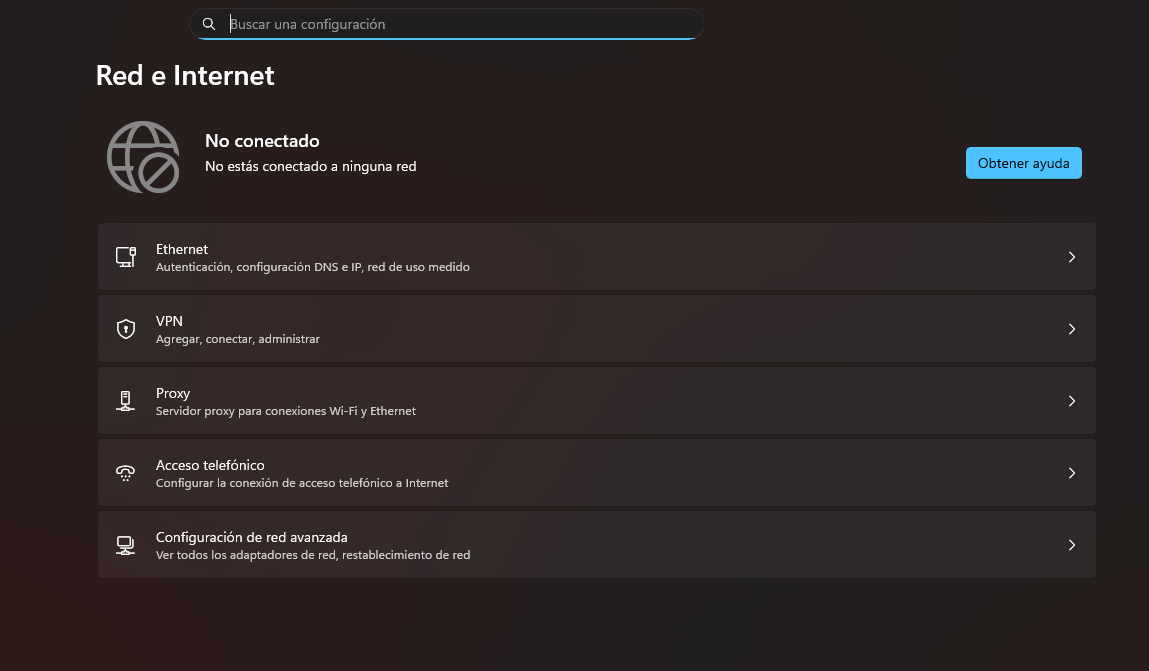
\includegraphics[width=0.68\textwidth]{img/E0.png}
  \caption{E0: equipo sin conexión de red al inicio de la sesión (panel ``Red e
  Internet'' de Windows, estado ``No conectado'').}
  \label{fig:e0}
\end{figure}

\section{Tabla de escenarios E0--E6}

\begin{table}[H]
\centering
\small
\renewcommand{\arraystretch}{1.12}
\begin{tabularx}{\textwidth}{@{}c >{\raggedright\arraybackslash}p{3.35cm} X@{}}
\toprule
\textbf{E} & \textbf{Escenario y evidencia} & \textbf{Interpretación} \\
\midrule
E0 &
Sin red al inicio. Panel de Red e Internet de Windows con el mensaje
``No conectado'' (figura~\ref{fig:e0}). &
La sesión comenzó sin conectividad. RMI sobre \cod{127.0.0.1} no necesita
Internet: el registro y las puertas pueden comunicarse por la interfaz de
bucle local. La captura acredita el aislamiento, aunque es el panel gráfico y
no la salida literal de \cod{Get-NetAdapter}. \\
\addlinespace
E1 &
Operación normal: entran personas por P1, P2 y P3; sale una por P2; la orden
\cod{estado} se consulta desde cada puerta. \sincaptura &
Las tres puertas consultan al mismo coordinador, por lo que el total que
devuelve \cod{estado} debe coincidir. Una salida decrementa el contador y no
puede dejar el valor por debajo de cero. La consistencia es inmediata porque
existe una sola copia del estado. \\
\addlinespace
E2 &
Aforo completo y token inválido: con aforo 10, la solicitud número 11 se
rechaza; después se envía una solicitud con un token incorrecto. \sincaptura &
El coordinador distingue dos motivos: \cod{aforo completo} y
\cod{token inválido}. El rechazo por token se escribe en la bitácora. Validar
el token antes de consultar el aforo evita revelar el estado interno a un
cliente no autenticado. \\
\addlinespace
E3 &
Carga concurrente: \cod{PruebaCarga} lanza 30 solicitudes \cod{ENTRAR}
simultáneas (10 hilos por puerta) con aforo 10, primero contra el coordinador
normal y luego contra el coordinador en modo \cod{-{}-inseguro}. \sincaptura;
cifras en la tabla~\ref{tab:e3}. &
En modo normal, la sección crítica garantiza exactamente 10 solicitudes
permitidas y 20 rechazadas; el contador termina en 10. En modo inseguro, la
lectura y la escritura están separadas por 50 ms: varias puertas leen el mismo
valor antes de que alguna escriba, se pierden actualizaciones y el número de
permitidas puede superar el aforo. \\
\addlinespace
E4 &
Puerta caída: se detiene P3; el coordinador debe marcarla como \textsc{caida}
en el tiempo fijado; al reiniciarla, debe marcarla de nuevo como
\textsc{activa}. \sincaptura &
El latido cada 2 s y el timeout de 6 s implementan un detector de fallos por
tiempo. La caída y la reactivación quedan registradas. El detector puede
producir falsos positivos si la red tarda más que el umbral, porque ``no llegó
el latido'' no equivale a ``la puerta está caída''. \\
\addlinespace
E5 &
Coordinador caído: con las puertas activas se detiene el coordinador y P1
intenta ejecutar \cod{entrar}. \sincaptura &
La puerta no puede completar \cod{procesar}: recibe una \cod{RemoteException}
y no admite a nadie localmente. El sistema prioriza no superar el aforo
(consistencia) sobre seguir atendiendo (disponibilidad); el público queda
bloqueado hasta que el coordinador vuelva. \\
\addlinespace
E6 &
Orden total: \cod{OrdenTotal} fusiona los registros de E1 a E5 y ordena por
Lamport y, en empate, por identificador. \sincaptura; no se conservó
\cod{orden\_total.log}. &
La relación envío$\to$recepción se conserva porque el receptor fija su reloj
en $\max(\text{local},\text{recibido})+1$. Los empates entre eventos
concurrentes se resuelven por identificador, lo que produce un orden total sin
alterar la causalidad. Los dos pares causales se detallan en la
tabla~\ref{tab:causales}. \\
\bottomrule
\end{tabularx}
\caption{Escenarios E0 a E6, evidencia disponible e interpretación.}
\label{tab:escenarios}
\end{table}

\section{Cifras de E3}

\begin{table}[H]
\centering
\small
\renewcommand{\arraystretch}{1.2}
\begin{tabularx}{\textwidth}{@{}l c c c c X@{}}
\toprule
\textbf{Modo} & \textbf{Solicitudes} & \textbf{Permitidas} &
\textbf{Rechazadas} & \textbf{Dentro al final} & \textbf{Lectura} \\
\midrule
Normal & 30 & 10 & 20 & 10 &
Cota que impone la exclusión mutua: la comprobación y el incremento son una
sola operación atómica. \\
\addlinespace
\cod{-{}-inseguro} & 30 & $>10$ (no determinista) & $<20$ & $>10$ &
Condición de carrera: lectura, pausa de 50 ms y escritura sin atomicidad;
varias puertas pueden leer el mismo cupo. \\
\bottomrule
\end{tabularx}
\caption{Cifras de E3 para 30 solicitudes simultáneas y aforo 10. La columna
``normal'' es la cota de diseño, no una medición: no se conservaron los
registros de la ejecución. En el modo inseguro no existe un valor único porque
depende del entrelazado de los hilos.}
\label{tab:e3}
\end{table}

En el modo normal los 30 hilos compiten por una única sección crítica: el
primero que encuentra \cod{dentro < 10} incrementa y recibe \cod{PERMITIDA};
cuando el contador llega a 10, el resto recibe \cod{RECHAZADA} por
\cod{aforo completo}. El resultado es 10 permitidas, 20 rechazadas y 10 dentro,
a costa de serializar la atención y convertir al coordinador en cuello de
botella. En el modo inseguro se lee, se esperan 50 ms y se escribe; varios
hilos leen el mismo valor antes de que alguno escriba y se pierden
actualizaciones. El número exacto depende del planificador, pero por diseño
puede superar 10 y llegar hasta 30: esa es la condición de carrera que el
\cod{synchronized} elimina.

\section{Dos pares causales de E6}

Lamport garantiza que si un evento $a$ precede causalmente a $b$, entonces
$L(a) < L(b)$. En el protocolo, el envío precede a la recepción y la respuesta
del coordinador precede a su recepción en la puerta. La
tabla~\ref{tab:causales} muestra dos pares con el formato del registro; los
valores son una traza de ejemplo, no un archivo conservado.

\begin{table}[H]
\centering
\small
\renewcommand{\arraystretch}{1.2}
\begin{tabularx}{\textwidth}{@{}c >{\raggedright\arraybackslash}p{3.7cm} c >{\raggedright\arraybackslash}p{3.7cm} c X@{}}
\toprule
\textbf{Par} & \textbf{Evento A} & \textbf{$L(A)$} & \textbf{Evento B} & \textbf{$L(B)$} & \textbf{Regla aplicada} \\
\midrule
1 & P1: \cod{ENVIAR;ENTRAR} & 4 & C: \cod{RECIBIR;ENTRAR} & 5 &
$L_C = \max(4, L_C)+1$ \\
\addlinespace
2 & C: \cod{ENVIAR;RESPUESTA} & 6 & P1: \cod{RECIBIR;RESPUESTA} & 7 &
$L_{P1} = \max(6, L_{P1})+1$ \\
\bottomrule
\end{tabularx}
\caption{Dos pares causales del protocolo. En \cod{orden\_total.log} la línea
del evento A debe aparecer antes que la del evento B; la ordenación por
$(\text{lamport},\text{id})$ respeta ambos pares.}
\label{tab:causales}
\end{table}

En el primer par, P1 incrementa su reloj antes de enviar y el coordinador lo
fija por encima al recibir; en el segundo, el coordinador incrementa al
responder y P1 lo fija al recibir. La ordenación por Lamport coloca
necesariamente $4$ antes que $5$ y $6$ antes que $7$. Si dos eventos
concurrentes empatan, el identificador decide el desempate sin alterar la
causalidad.

\section{Respuestas a las preguntas de análisis}

\subsection*{1. ¿Por qué el modo \cod{-{}-inseguro} permitió más entradas que el aforo? ¿Qué mecanismo evita el desborde y qué costo tiene?}

En el diseño, el modo normal impone exclusión mutua: \cod{procesar} está
sincronizado y la comprobación y el incremento son una sola operación atómica;
con 30 hilos y
aforo 10 la cota es 10/20/10. El costo es la serialización: las puertas esperan
y el coordinador se vuelve cuello de botella. El modo \cod{-{}-inseguro} separa
lectura y escritura con 50 ms de pausa; varios hilos leen el mismo
\cod{dentro}, todos creen que hay cupo y se pierden actualizaciones. Esa es la
condición de carrera que el \cod{synchronized} elimina; no se conservaron las
cifras, así que 10/20/10 es la cota de diseño, no una medición.

\subsection*{2. En E5, ¿qué priorizó el sistema, la consistencia del aforo o la disponibilidad de las puertas?}

Se priorizó la consistencia del aforo (C) sobre la disponibilidad (A). Si el
coordinador no responde, la puerta no tiene una copia autorizada del contador
y no admite a nadie: \cod{procesar} lanza una \cod{RemoteException} y la puerta
informa que el coordinador no está disponible. Es una decisión CP: ante una
partición, se prefiere rechazar antes que arriesgar un sobreaforo. Para el
público, la entrada se detiene mientras dure el fallo; para la administración,
se pierde el servicio pero se conserva la garantía legal del aforo y la
trazabilidad de los rechazos. La alternativa AP (admitir con un contador local
y reconciliar después) daría disponibilidad a costa de poder superar el aforo.

\subsection*{3. El coordinador es un punto único de fallo. ¿Qué mecanismo usaría para que el sistema siga funcionando y qué problema nuevo aparecería?}

Replicaría el coordinador con un líder elegido mediante Bully o Raft y haría
que las puertas redirijan las solicitudes al nuevo líder; el estado
\cod{dentro} y los registros también tendrían que replicarse. El problema
nuevo es la consistencia del contador replicado: si hay una partición, dos
réplicas pueden creerse líderes y admitir en paralelo (\emph{split-brain}),
duplicando entradas o superando el aforo. Se necesita una mayoría o quórum para
aceptar escrituras, lo que reduce la disponibilidad durante la partición y
añade latencia. Además hay que definir la idempotencia de las solicitudes en
vuelo y transferir el estado al nuevo líder sin perder eventos.

\subsection*{4. ¿Qué falacia tuvo en cuenta al fijar los tiempos de 2 y 6 segundos? ¿Qué pasaría con una latencia de 7 segundos?}

La falacia es ``la red es fiable'' (y su pariente ``la latencia es cero o está
acotada''). Los 2 s de latido y los 6 s de timeout suponen que un latido llega
en menos de 6 s. Con una latencia de 7 s, todos los latidos llegan después del
umbral: el coordinador marcaría las tres puertas como \textsc{caidas} aunque
estén vivas y, al recuperarse la red, las marcaría como \textsc{activas},
produciendo una oscilación de estados. Si se aumenta el timeout, la detección
se vuelve más lenta. La solución es un timeout adaptativo con varios intentos,
jitter y no interpretar ``no llegó'' como ``está caído''.

\section{Limitaciones y conclusión}

La evidencia disponible se limita a E0: no se conservaron capturas ni
registros de E1 a E6, de modo que las cifras de E3 y los pares de E6 son cotas
de diseño y no mediciones. A esto se suma que \cod{CoordinadorServicio} no
implementa todavía \cod{procesar}, por lo que el prototipo no se puede ejecutar
de extremo a extremo. Completar esa implementación y repetir los escenarios es
el trabajo inmediato; el diseño presentado permite hacerlo sin cambiar el
contrato ni la configuración.

\end{document}
